
\documentclass{beamer}


\mode<presentation>
{
  \usetheme{CambridgeUS}
	\usecolortheme{beaver}
  % or ...

  \setbeamercovered{transparent}
  % or whatever (possibly just delete it)
}


\usepackage{xeCJK}
\usepackage[english]{babel}
\usepackage[utf8]{inputenc}
\usepackage{times}
\usepackage[T1]{fontenc}
\usepackage{hyperref}
\usepackage{pifont}
\usepackage{bibentry}
\usepackage{verbatim}
\usepackage{color}
\newcommand{\cmark}{\ding{51}}%
\newcommand{\xmark}{\ding{55}}%
\setCJKmainfont{WenQuanYi Micro Hei}
\renewcommand{\raggedright}{\leftskip=0pt \rightskip=0pt plus 0cm}
\raggedright

\let\oldfootnotesize\footnotesize
\renewcommand*{\footnotesize}{\oldfootnotesize\tiny}


\title[开源软件基础] 
{开源软件基础}
\subtitle{利用Stack Overflow}

\author[Zhilei Ren] 
{Zhilei Ren}

\institute[OSCAR Team] % (optional, but mostly needed)
{
\\
\includegraphics[width=0.2\textwidth]{../../utils/logo.jpg}\\
OSCAR Team, School of Software, 
Dalian University of Technology
}


\subject{Open source}



\pgfdeclareimage[height=0.5cm]{university-logo}{../../utils/logo.jpg}
\logo{\pgfuseimage{university-logo}}



% Delete this, if you do not want the table of contents to pop up at
% the beginning of each subsection:
\AtBeginSubsection[]
{
  \begin{frame}<beamer>{Outline}
    \tableofcontents[currentsection,currentsubsection]
  \end{frame}
}


% If you wish to uncover everything in a step-wise fashion, uncomment
% the following command: 

%\beamerdefaultoverlayspecification{<+->}

\setbeamertemplate{section in toc}[circle]
\setbeamertemplate{items}[circle]
\setbeamertemplate{caption}[numbered]
\setbeamertemplate{bibliography item}{\insertbiblabel}
\setbeamertemplate{bibliography entry title}{}
\setbeamertemplate{bibliography entry journal}{}

\begin{document}

\begin{frame}
  \titlepage
\end{frame}

%\begin{frame}{Outline}
%  \tableofcontents[currentsection,currentsubsection, 
%    hideothersubsections, 
%    sectionstyle=show,
%]
%\end{frame}

\AtBeginSection[]
{
 \begin{frame}<beamer>
 \frametitle{Outline}
 \tableofcontents[currentsection]
 \end{frame}
}

\section{Stack Overflow简介}
\begin{frame}[t]{Stack Overflow简介}
     \begin{block}{Stack Overflow}
		 \scriptsize
		 Stack Overflow是一个程序设计领域的问答网站，隶属Stack Exchange Network。网站允许注册用户提出或回答问题，利用积分制度让用户自行管理。另外网站也会根据用户的贡献颁发徽章。用户创建的内容都使用知识共享协议授权。直至2018年9月，Stack Overflow有超过9,400,000名注册用户和超过16,000,000个问题，其中最常见的主题有JavaScript、Java、C\#、PHP、Android、Python、jQuery和HTML\footnote{\url{https://zh.wikipedia.org/zh-cn/Stack_Overflow}}
     \end{block}
\end{frame}

\begin{frame}[t]{Stack Overflow}
	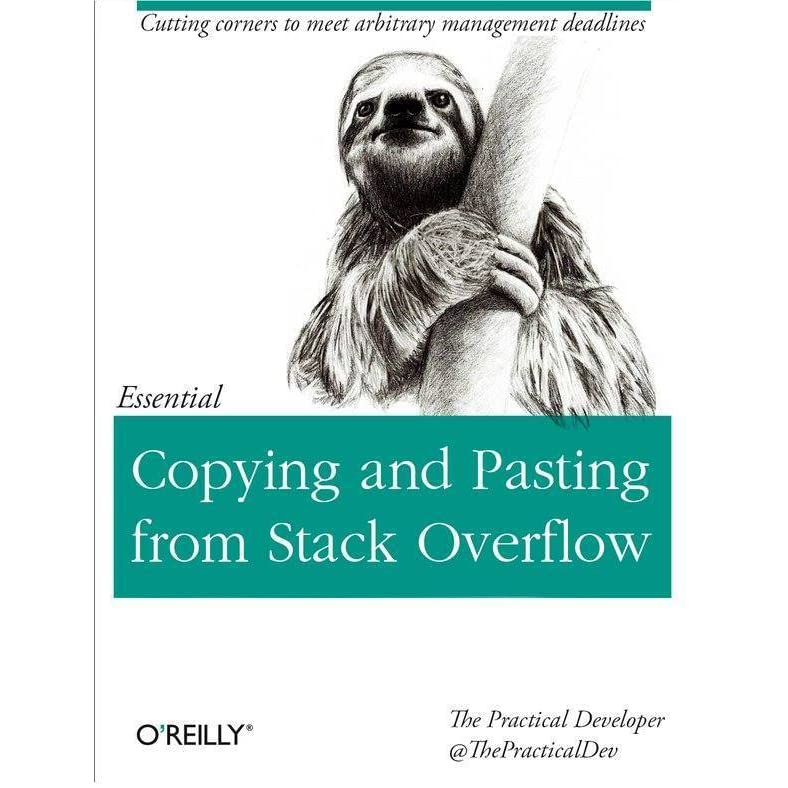
\includegraphics[width=.4\textwidth]{stackoverflow.jpg}
	
\end{frame}

\begin{frame}[t]{Stack Overflow}
	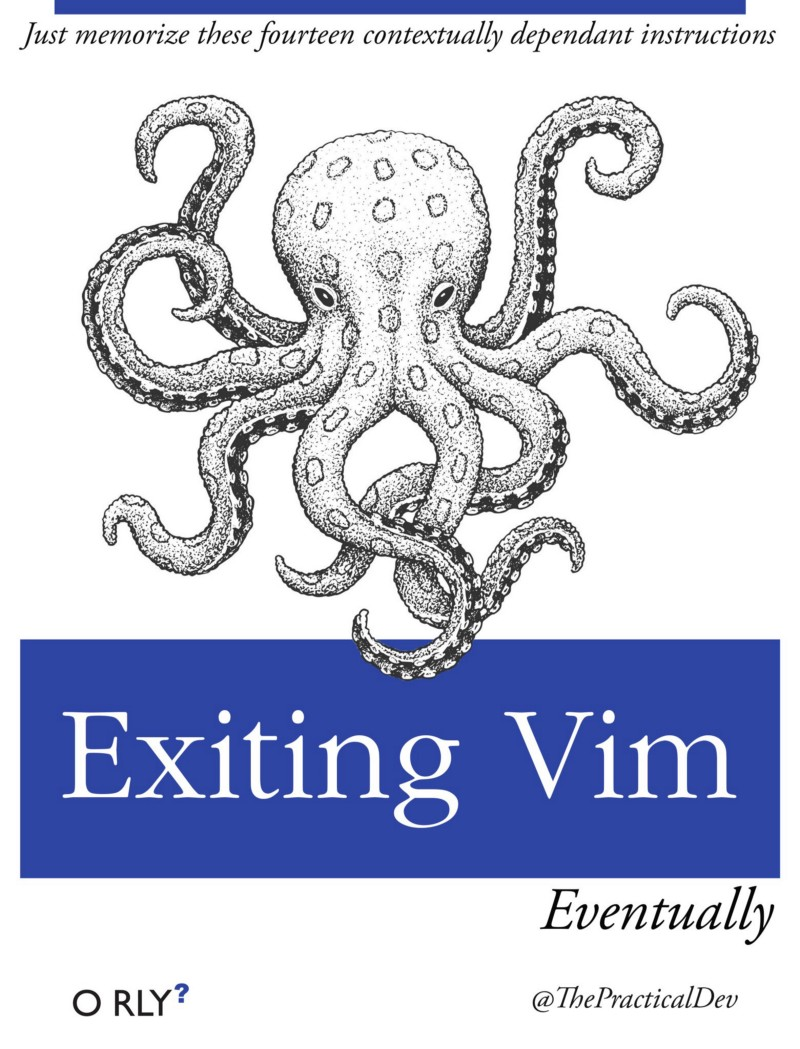
\includegraphics[width=.4\textwidth]{vim.jpeg}

	How do I exit the Vim editor\footnote{\url{https://stackoverflow.com/questions/11828270/how-do-i-exit-the-vim-editor}}
	
\end{frame}

\begin{frame}[t]{Stack Overflow}
	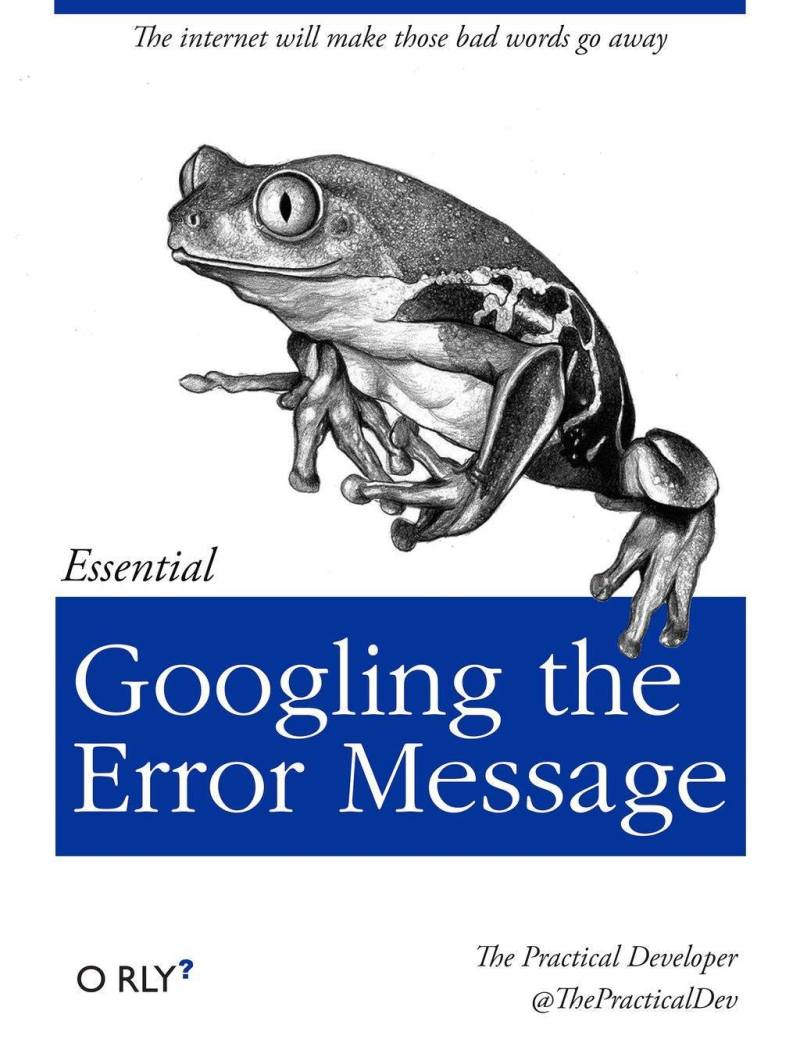
\includegraphics[width=.4\textwidth]{google.jpg}
	
\end{frame}
\begin{frame}[t]{Stack Overflow}
	
\includegraphics[width=.4\textwidth]{latex.jpg}
	
\end{frame}
\begin{frame}[t]{Stack Overflow简介}
     \begin{block}{技术}
		 \scriptsize
		 Stack Overflow是以ASP.NET 3.5撰写而成并使用ASP.NET MVC（MVC模式）框架。 未注册用户可以访问网站的大部分功能，使用OpenID登录的用户可以使用更多功能，诸如：创建个人文件、赚取声望点数并激活修改标签或者投票关闭问题。
     \end{block}
\end{frame}

\begin{frame}[t]{Stack Overflow}
     \begin{block}{声望值和管理制度}
		 \scriptsize
利用“声望值”来决定用户的管理权限，以此达到社区自我管理。声望值（Reputation）就是用户进行网站交互时能获取的分数，例如，用户 A 回答了一个问题，用户 B 对用户 A 的解答给予了“加分”，用户 A 就会因而获得10点声望值。对已有问题或答案扣分，作者和评价者的声望值都会降低，以此避免恶意报复。当声望值达到某个程度，用户的权限（Privileges）就会增加，如声望值超过50点就可以评论答案、声望值超过 2000 可以直接编辑问题，无需作者同意。虽然“声望值”很大程度能让社区高效的自我管理，但是声望值机制并非完美。例如用户询问或回答新手常遇到的简单问题（在有大量的用户的语言），就很容易获得非常多的声望值，导致他们获得不符合自身能力的 Privileges。

用户可以提交编辑标题、提交编辑主题标签、提交编辑问题内文（如果声望值不够高，就需要发问者接受编辑）。并且能够将问题的状态标示为重复问题、低质量问题、删除（标示为被删除）问题、关闭问题，让社区的问答维持质量。在 2016 年，社区删除了 150 万个帖子，其中大约 8\% 是由版主删除的。
     \end{block}
\end{frame}
\section{How do I ask a good question}
\begin{frame}[t]{How to ask question\footnote{\url{https://stackoverflow.com/help/how-to-ask}}}
	\begin{enumerate}
		\item Write a title that summarizes the specific problem
		\item Introduce the problem before you post any code
		\item Help others reproduce the problem
		\item Include all relevant tags
		\item Proof-read before posting!
		\item Post the question and respond to feedback
	\end{enumerate}
\end{frame}

\begin{frame}[t]{What to avoid asking}
To prevent your question from being flagged and possibly removed, avoid asking subjective questions where …

\begin{enumerate}
	\item every answer is equally valid: “What’s your favorite \_\_\_\_\_\_?”
    \item your answer is provided along with the question, and you expect more answers: “I use \_\_\_\_\_\_ for \_\_\_\_\_\_, what do you use?”
    \item there is no actual problem to be solved: “I’m curious if other people feel like I do.”
    \item you are asking an open-ended, hypothetical question: “What if \_\_\_\_\_\_ happened?”
    \item your question is just a rant in disguise: “\_\_\_\_\_\_ sucks, am I right?”
\end{enumerate}
	
\end{frame}

\section{Stack Overflow Survey}
\begin{frame}[t]{The Beloved}
Rust held onto it's spot as the most beloved language among the professional developers we surveyed. That said, the majority of developers who took the survey aren't familiar with the language\footnote{\url{https://stackoverflow.blog/2020/05/27/2020-stack-overflow-developer-survey-results/}}.

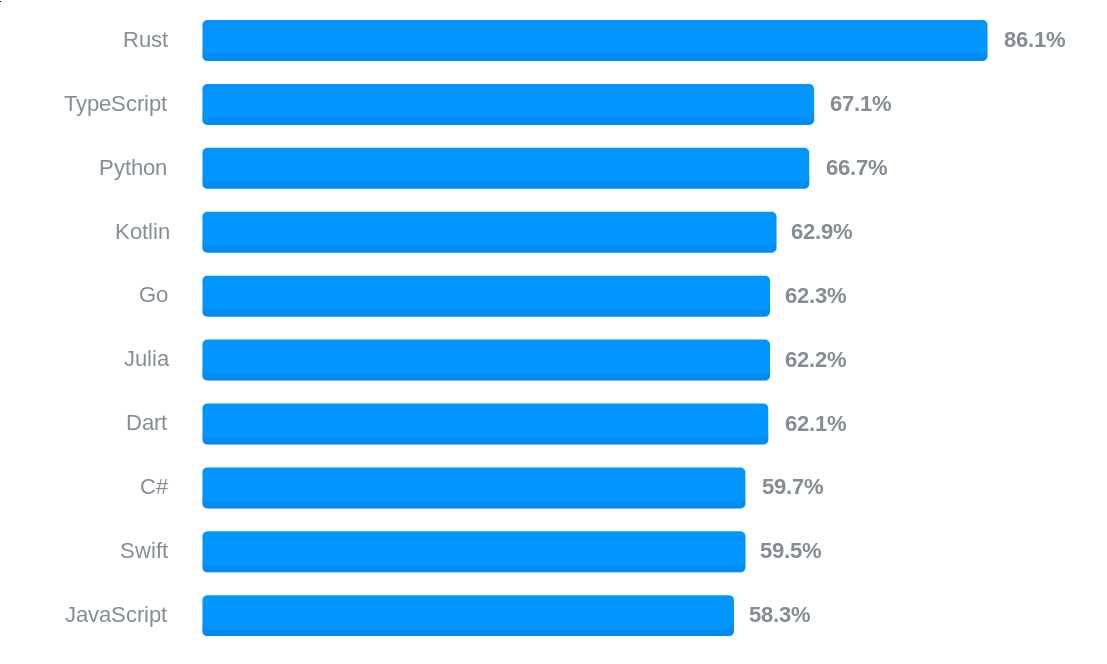
\includegraphics[width=.6\textwidth]{rank.png}
	
\end{frame}

\section{Something Interesting}
\label{sec:Something Interesting}

\begin{frame}[t]{StackSort}
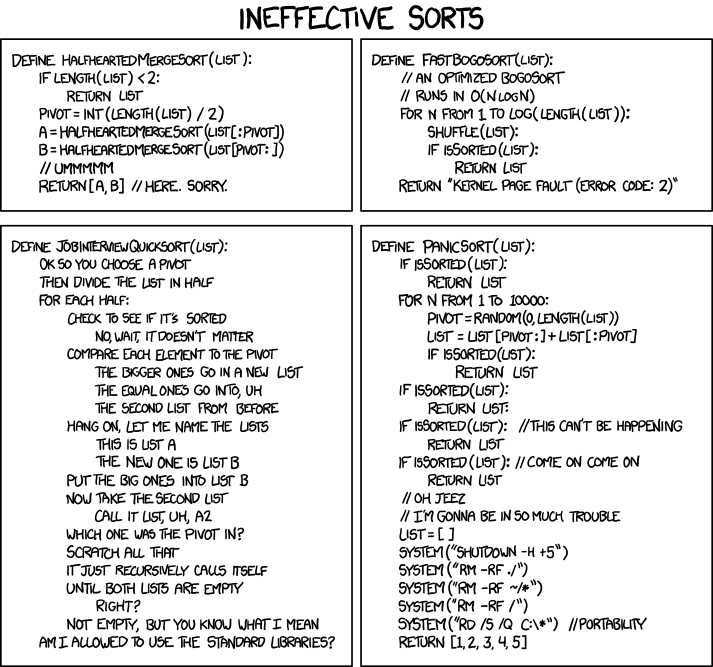
\includegraphics[width=.5\textwidth]{stacksort.png}	

\scriptsize

StackSort connects to StackOverflow, searches for "sort a list", and downloads and runs code snippets until the list is sorted\footnote{\url{https://xkcd.com/1185/}}. JS\footnote{\url{http://gkoberger.github.io/stacksort/}}/Python implementation \footnote{\url{https://pypi.org/project/stacksort/}}
\end{frame}
\begin{frame}[t,fragile]{StackSort}

\begin{verbatim}
>>> from stacksort import quicksort
>>> quicksort([1, 3, 2, 4])
[1, 2, 3, 4]
>>> from stacksort import heap_sort
>>>heap_sort([1, 2, 4, 3])
[2, 3, 4]

\end{verbatim}
	
\end{frame}


\end{document}
